\documentclass[conference]{IEEEtran}
\IEEEoverridecommandlockouts

\usepackage{cite}
\usepackage{amsmath,amssymb,amsfonts}
\usepackage{algorithm}
\usepackage{algpseudocode}
\usepackage{graphicx}
\usepackage{booktabs}
\usepackage{array}
\usepackage{url}
\usepackage{hyperref}
\usepackage{tikz}
\usetikzlibrary{arrows.meta,positioning,shapes.geometric,fit,calc}
\usepackage{balance}

\hypersetup{hidelinks}
\graphicspath{{figures/}}

\title{A Camera-Geometry and Body-Proportion Approach for Image-Based Human Height and Weight Estimation}

\author{
\IEEEauthorblockN{Author Name 1, Author Name 2, Author Name 3}
\IEEEauthorblockA{\textit{School/Department of Department Name}\\
\textit{Institution Name}\\
City, Country\\
author email(s)}
}

\begin{document}
\maketitle

\begin{abstract}
This paper presents a full-stack prototype for estimating human height and weight from full-body images. The system combines YOLOv8 person detection, MediaPipe pose and segmentation, pinhole-camera geometry, Ridge height calibration, and Random Forest weight regression, with a React interface and FastAPI service. On an 84-image training cohort from 22 participant IDs, nested participant-grouped cross-validation achieved height MAE of 3.92 cm and weight MAE of 5.92 kg, compared with participant-level median baselines of 7.31 cm and 9.95 kg, respectively. A separate 36-image cohort grouped by normalized names (24 groups) produced 6.85 cm calibrated-height MAE and 8.95 kg weight MAE; in that cohort, the height median baseline was slightly better (6.68 cm), while the weight baseline MAE was 11.12 kg. These are cross-validation results on small project datasets, not external test performance; name-based grouping may miss aliases, and the two cohorts are not asserted to contain disjoint people. The prototype is not a validated measurement instrument.
\end{abstract}

\begin{IEEEkeywords}
human height estimation, weight estimation, computer vision, YOLOv8, MediaPipe Pose, pinhole camera model, Random Forest regression, FastAPI
\end{IEEEkeywords}

\section{Introduction}
Estimating body measurements from images is a computer-vision problem with potential applications in contactless measurement, interactive systems, and preliminary anthropometric assessment. Directly recovering metric height from a two-dimensional image is challenging because pixel coordinates depend on camera geometry, subject distance, camera orientation, posture, occlusion, and landmark localization. Weight estimation is more ambiguous: a single image does not directly reveal body depth, tissue composition, or other variables needed to determine mass.

The supplied implementation addresses these two tasks differently. Height is first estimated from detected body boundaries using a pinhole-camera projection model. A saved regression calibration model can then compensate for systematic error observed in the labelled camera setup. Weight is predicted from calibrated height and seven visible body-proportion or silhouette features using a saved Random Forest regressor. An optional side-view image is processed independently and its weight prediction is averaged with the front-view prediction.

The implementation includes a React/Vite frontend and a FastAPI backend. The backend loads YOLOv8, MediaPipe Pose, and MediaPipe Selfie Segmentation at startup, processes uploaded images, calculates measurements, and returns image overlays. This paper documents the implementation that is present in the supplied archive, rather than the earlier design notes alone.

\subsection{Problem Statement}
Given a full-body image and user-supplied camera height and subject distance, estimate the subject's height in centimetres and feet/inches. In addition, estimate weight in kilograms from visible body proportions and, optionally, combine estimates from front and side views. The system must return a visual explanation of the detected person and measurement landmarks.

\subsection{Objectives and Contributions}
The project objectives supported by the implementation are:
\begin{itemize}
  \item detect a dominant person in an uploaded image using YOLOv8;
  \item extract body landmarks using MediaPipe Pose and estimate head-top and ground-contact pixel coordinates;
  \item convert image coordinates into a metric height estimate using pinhole-camera geometry and camera metadata;
  \item apply a learned height-calibration model and estimate weight with a Random Forest regressor using normalized body-shape features;
  \item expose prediction and feedback endpoints through FastAPI and present annotated outputs in a React interface; and
  \item evaluate the height and weight regressors with participant-grouped cross-validation, compare them with participant-level median baselines, and state the remaining limits on generalization.
\end{itemize}
The contribution is an implementation and integration of these components, together with nested participant-grouped evaluation on the model-training cohort and a separate name-grouped evaluation on an additional labelled image cohort. The supplied files do not establish a novel computer-vision algorithm or a validated clinical measurement method.

\section{Related Work}
The twelve studies supplied in the literature-review spreadsheet cover image-based prediction, geometric measurement, clinical anthropometry, 3D body reconstruction, multi-task learning, motion sensing, and broader surveys. They differ in target variable, input modality, dataset, and evaluation protocol; therefore, their reported errors should not be treated as a directly comparable leaderboard.

Jin \textit{et al.} estimate body mass index (BMI) from a single image by combining explicitly designed anthropometric proportions with deep visual features learned by a ResNet-101 branch \cite{jin2023}. This work is relevant to extracting body-shape cues from images, but BMI is not the same target as weight in kilograms. Jiang and Guo likewise analyze body images, using body contours and joint points to derive five features before applying support-vector regression (SVR) and Gaussian-process regression (GPR) to estimate BMI \cite{jiang2019}. Their work supports the use of interpretable body proportions, while also highlighting the distinction between BMI prediction and direct weight estimation.

Suwatkittiwong \textit{et al.} investigate height measurement using a known square template placed on the ground, using the template as a geometric scale reference \cite{suwat2018}. This is closely related to geometry-based measurement, but requires a known reference object in the scene. In a clinical setting, Melo \textit{et al.} compare formula-based estimates of height and weight with measured values for hospitalized adults \cite{melo2014}. Their equations rely on physical anthropometric measurements, so the method is not a raw-image-only pipeline.

For infants, Shu \textit{et al.} study height and weight estimation from a single image, comparing CNN backbones for height and single-task and multi-task MobileNet-based methods for weight, with five-fold cross-validation \cite{shu2023}. The target population and image conditions differ from those of a general full-body adult system. Thakkar and Farid examine the feasibility of forensic height and weight estimation using fitted 3D human pose and body models \cite{thakkar2021}. Their analysis emphasizes the uncertainty caused by pose, view angle, image quality, and ambiguity between apparent image size and true physical scale.

Altinigne \textit{et al.} propose estimating height and weight from unconstrained full-body images using a multi-task U-Net framework that predicts body silhouettes and skeletal joints alongside the measurements \cite{altinigne2020}. Unlike the current implementation, their method does not require user-provided camera distance and camera height. Han \textit{et al.} address height and weight estimation from facial images through multi-task learning, using ResNet-50 and auxiliary age-estimation and gender-classification tasks to support the main regression tasks \cite{han2020}. Their facial-image input and auxiliary labels differ from the current system's full-body front/side images and camera metadata.

Maganti \textit{et al.} describe estimation from virtual visuals using OpenCV and MediaPipe/BlazePose landmarks, with interpupillary distance as a scale reference and regression methods for prediction \cite{maganti2022}. Their paper reports results on its own evaluation data; those results are not results of the present project. Rativa \textit{et al.} compare linear regression, SVR, GPR, and feed-forward neural-network regression using measured anthropometric variables from NHANES III and the U.S. Army Anthropometry Survey \cite{rativa2018}. This work informs the choice of regression approaches, but requires anthropometric measurements rather than extracting them directly from RGB images.

Dong and Cai estimate height and weight from walking-related motion data captured by a smartphone and smart band. They combine motion features using Serial+CC fusion and compare several regression and sequence models \cite{dong2025}. This provides a non-image-based point of comparison; the current system instead uses front and side images with camera metadata. Finally, Jan \textit{et al.} survey body-weight-estimation methods, datasets, applications, and limitations across anthropometric equations, imaging, depth sensing, and learning-based methods \cite{jan2025}. As a survey, it synthesizes findings from different experimental settings rather than reporting one new model result.

\subsection{Positioning of the Present Work}
Across these studies, some approaches need reference objects, physical measurements, facial images, 3D reconstruction, or wearable motion data. The present implementation combines two full-body views with camera height and subject distance; estimates height through camera geometry followed by learned Ridge calibration; and predicts weight from calibrated height and visible body-proportion/silhouette features using a Random Forest regressor. The grouped evaluations reported here are initial benchmarks on the available cohorts, not verified external subject-independent tests; they do not establish superiority over prior methods.

\subsection{Research Gap}
The reviewed papers use different target variables (including BMI rather than weight), populations, sensors, image types, and evaluation splits. These differences limit direct comparison of published error values. To address the project's immediate evaluation gap, we report out-of-fold errors under participant-name grouping and compare weight predictions with a training-fold median baseline. This is stronger than an image-level random split, but it is not a definitive subject-independent benchmark: grouping is based on normalized name strings, possible aliases remain, and the cohort is small. The results are therefore presented as preliminary estimates, not evidence of superiority or deployment readiness.

\section{System Overview}
Fig.~\ref{fig:architecture} summarizes the implemented service architecture. The frontend submits multipart image data and camera parameters to the API. The backend runs person detection, pose estimation, geometric measurement, feature extraction, height calibration, and weight regression. Annotated images and estimates are returned as JSON.

\begin{figure*}[t]
\centering
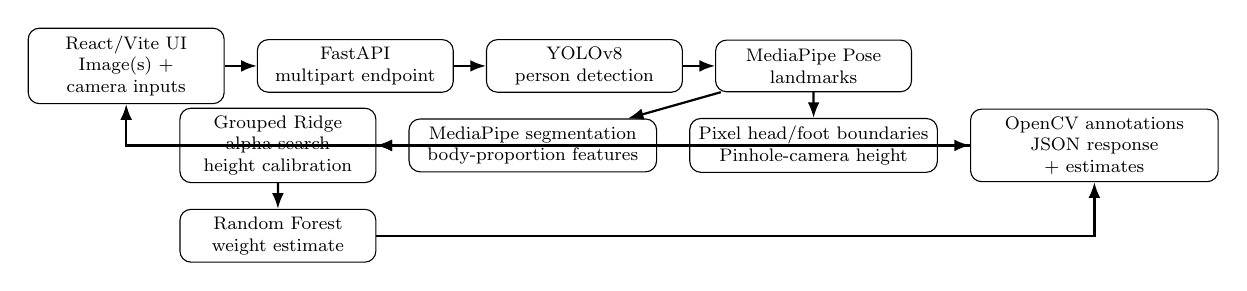
\begin{tikzpicture}[scale=0.82, transform shape,
  node distance=4mm and 5mm,
  block/.style={draw, rounded corners, align=center, minimum height=8mm, text width=28mm, font=\footnotesize},
  wide/.style={draw, rounded corners, align=center, minimum height=8mm, text width=36mm, font=\footnotesize},
  arr/.style={-{Latex[length=2mm]}, thick}
]
\node[block] (ui) {React/Vite UI\\Image(s) + camera inputs};
\node[block, right=of ui] (api) {FastAPI\\multipart endpoint};
\node[block, right=of api] (yolo) {YOLOv8\\person detection};
\node[block, right=of yolo] (pose) {MediaPipe Pose\\landmarks};
\node[wide, below=of pose] (geom) {Pixel head/foot boundaries\\Pinhole-camera height};
\node[wide, left=of geom] (feat) {MediaPipe segmentation\\body-proportion features};
\node[block, left=of feat] (cal) {Grouped Ridge alpha search\\height calibration};
\node[block, below=of cal] (rf) {Random Forest\\weight estimate};
\node[wide, right=of geom] (out) {OpenCV annotations\\JSON response + estimates};
\draw[arr] (ui)--(api);
\draw[arr] (api)--(yolo);
\draw[arr] (yolo)--(pose);
\draw[arr] (pose)--(geom);
\draw[arr] (pose)--(feat);
\draw[arr] (geom)--(cal);
\draw[arr] (feat)--(cal);
\draw[arr] (cal)--(rf);
\draw[arr] (geom)--(out);
\draw[arr] (rf.east) -| (out.south);
\draw[arr] (out.west) -| (ui.south);
\end{tikzpicture}
\caption{Architecture reconstructed from the supplied backend and frontend source code.}
\label{fig:architecture}
\end{figure*}

\section{Methodology}
\subsection{Person Detection}
The backend loads the configured YOLOv8 model, with \texttt{yolov8n.pt} as the configured model path. Detections are filtered to the COCO person class (class identifier 0) and confidence threshold 0.4. If multiple people pass the filter, the implementation selects the bounding box with the largest area. This design targets the dominant person and may be unsuitable when the intended subject is not the largest person in the frame.

\subsection{Pose Landmark Extraction and Pixel Boundaries}
MediaPipe Pose is applied to a padded crop around the selected detection. The implementation converts normalized landmark coordinates into image coordinates and uses the left/right ears, shoulders, hips, knees, ankles, heels, and toes. The head-top estimate is formed by extrapolating above the midpoint of the ears by 1.2 times the absolute vertical difference between the ear midpoint and shoulder midpoint:
\begin{equation}
y_{\mathrm{top}} = y_{\mathrm{ears}} -
1.2\left|y_{\mathrm{shoulders}}-y_{\mathrm{ears}}\right|.
\label{eq:headtop}
\end{equation}
The bottom boundary is the largest image-coordinate $y$ among the left/right heel and toe landmarks:
\begin{equation}
y_{\mathrm{bottom}}=\max(y_{\mathrm{heel,L}},y_{\mathrm{heel,R}},
y_{\mathrm{toe,L}},y_{\mathrm{toe,R}}).
\label{eq:bottom}
\end{equation}
The vertical pixel span is
\begin{equation}
p_h = |y_{\mathrm{bottom}}-y_{\mathrm{top}}|.
\label{eq:pixelheight}
\end{equation}
The pipeline rejects images when this span is below 10 pixels. A posture warning is raised when either computed knee angle is below $160^\circ$.

\subsection{Pinhole-Camera Height Estimation}
Let $H_I$ be the image height in pixels, $v$ the configured vertical field of view, and $f_y$ the vertical focal length in pixel units. The implementation computes
\begin{equation}
f_y = \frac{H_I/2}{\tan(v/2)}.
\label{eq:focal}
\end{equation}
Angles relative to the image's optical centre are
\begin{align}
\alpha_t &= \tan^{-1}\left(\frac{H_I/2-y_{\mathrm{top}}}{f_y}\right),\\
\alpha_b &= \tan^{-1}\left(\frac{H_I/2-y_{\mathrm{bottom}}}{f_y}\right).
\end{align}
Given subject distance $D$ and camera height $C$, the ray to the ground-contact point is used to infer camera pitch:
\begin{align}
\theta_b &= -\tan^{-1}(C/D),\\
\theta &= \theta_b-\alpha_b,\\
\phi_t &= \theta+\alpha_t.
\end{align}
The geometric height estimate is then
\begin{equation}
\widehat{H}_{g} = \max\{0,\ C+D\tan(\phi_t)\}.
\label{eq:height}
\end{equation}
This equation follows the implementation in \texttt{height\_estimator.py}. It assumes the supplied camera-to-subject distance is appropriate for the subject and that the lowest detected heel/toe point represents ground contact. Camera pitch is inferred from that ground-contact assumption; camera height, distance, field of view, posture, and landmark accuracy therefore influence the result.

\subsection{Body-Proportion Features}
The implementation derives eight inputs for the regressors. Let $w_b$ and $h_b$ denote bounding-box width and height; $p_h$ is the detected pixel height. Shoulder and hip widths are Euclidean distances between the corresponding left/right landmarks. A segmentation mask is thresholded at 0.5 inside the person bounding box. The features are:
\begin{align}
x_1 &= \widehat{H}_{g}, \quad
x_2 = \frac{w_{\mathrm{shoulder}}}{p_h}, \quad
x_3 = \frac{w_{\mathrm{hip}}}{p_h},\\
x_4 &= \mathrm{mean}(\mathrm{person\ mask}), \quad
x_5 = \frac{w_b}{h_b},\\
x_6 &= \frac{n_{0.30}}{p_h}, \quad
x_7 = \frac{n_{0.52}}{p_h}, \quad
x_8 = \frac{n_{0.70}}{p_h},
\end{align}
where $n_r$ is the number of foreground pixels in the mask row at relative vertical position $r$. The row widths approximate chest-, waist-, and lower-body-level silhouette widths. These are image-derived proxies and should not be interpreted as calibrated physical circumferences.

\subsection{Height Calibration}
The originally supplied inference artifact is a \texttt{StandardScaler}--\texttt{RidgeCV} pipeline. In the revised training workflow and the grouped results in this paper, we use a \texttt{StandardScaler}--Ridge pipeline with alpha selected from $\{0.1,1,10,100\}$ by grouped cross-validation MAE within each training partition. Nested out-of-fold calibrated heights are used when fitting the weight model, avoiding in-sample height predictions as training features. The metrics evaluate this fold-specific refitting procedure, not a frozen external test of the originally supplied inference artifact. At application inference, the calibrated estimate replaces the geometric estimate for displayed height and weight prediction.

\subsection{Weight Estimation}
The evaluated weight model is a \texttt{RandomForestRegressor} configured with 300 trees, \texttt{min\_samples\_leaf=2}, \texttt{max\_features=0.8}, and random seed 42. It predicts weight from the eight features in the previous subsection. In each evaluation, the regressor is fit separately within each outer training fold using only that cohort; calibrated height inputs for training records are generated out of fold, and test folds hold out complete groups. The 36-image evaluation uses normalized names, while the separate training-cohort evaluation uses the \texttt{person\_id} field. Within each fold, multiple images per participant remain repeated training observations; final metrics average predictions within participant before scoring, so each group contributes equally to the reported metric.

At inference, the model predicts weight in kilograms. If the model exposes individual tree predictions, the code defines a spread as the larger of 4 kg and 1.5 times the standard deviation across tree predictions; otherwise, it uses 8 kg. The output interval is the prediction plus/minus this spread, clipped at zero on the lower end. This is an implementation-defined heuristic, not a statistically calibrated prediction interval.

If a side-view image is supplied, the backend processes it through the same pipeline and averages the front- and side-view weight predictions. The corresponding reported range endpoints are averaged as well. The primary displayed height remains based on the primary uploaded image.

\subsection{API and User Interface}
The FastAPI service exposes \texttt{/api/predict-body}, \texttt{/api/submit-feedback}, and \texttt{/api/models/info}, as well as root and health-check endpoints. Prediction requests use multipart form data. Responses include estimated height, geometric height, confidence score, bounding box, pixel height, camera metadata, weight estimate, approximate weight range, and base64-encoded annotated images. OpenCV overlays include a bounding box, pose connections, measurement endpoints, and a height label. The frontend is implemented using React, Vite, Axios, and Lucide React.

The feedback endpoint appends submitted labels and images to the first dataset and schedules retraining. This mechanism requires governance before deployment: consent, access controls, data-quality checks, duplicate management, and a reproducible versioned training process should be addressed.

\begin{figure*}[t]
\centering
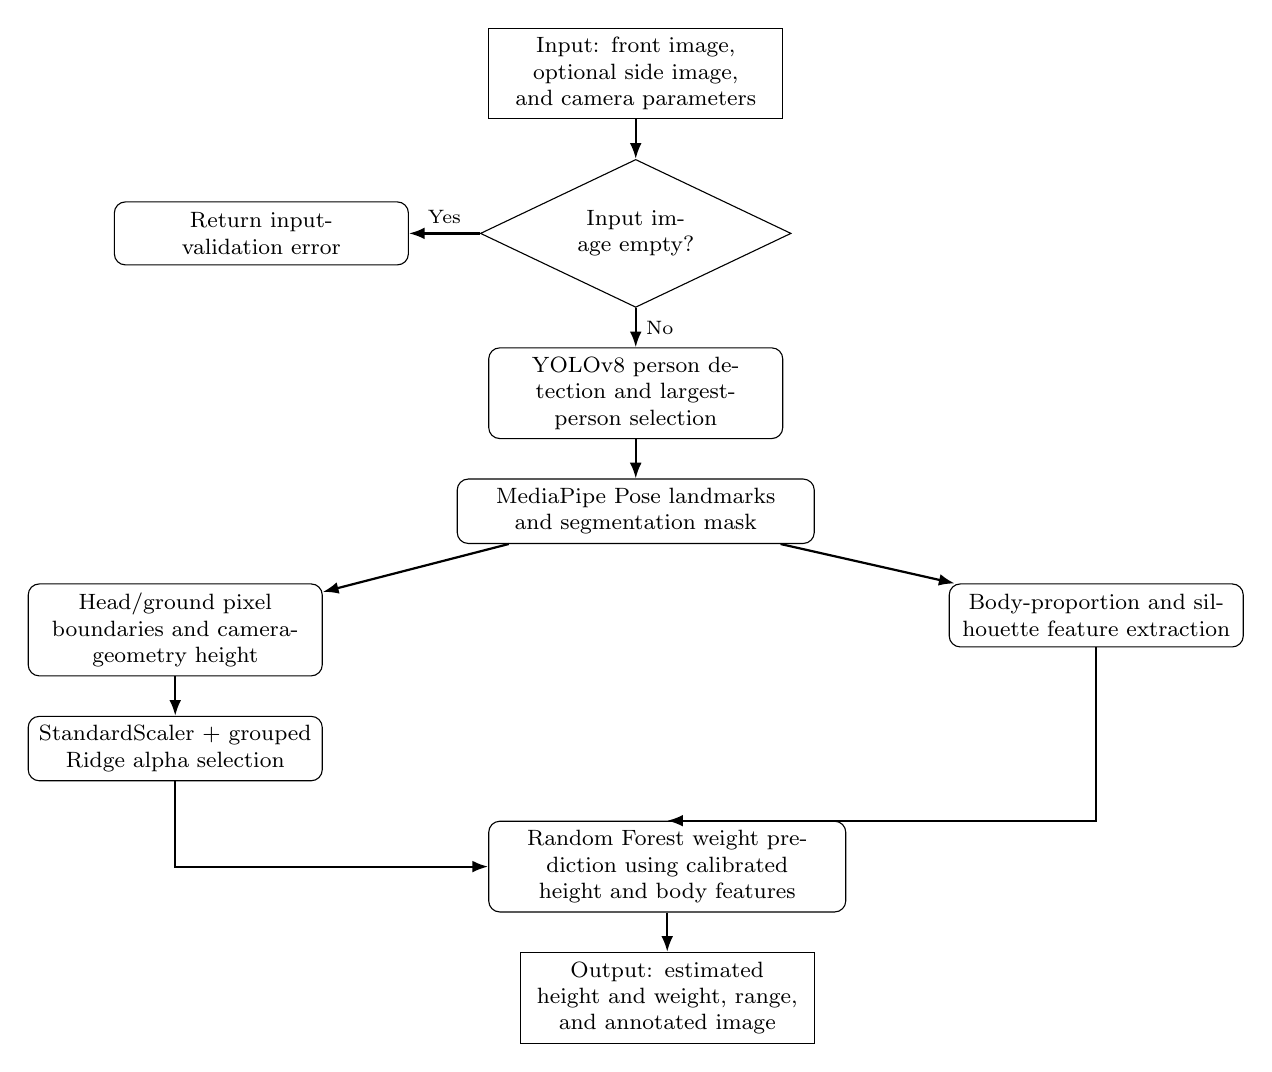
\begin{tikzpicture}[
  node distance=5mm and 9mm,
  process/.style={draw,rounded corners,align=center,text width=35mm,minimum height=8mm,font=\footnotesize},
  wide/.style={draw,rounded corners,align=center,text width=43mm,minimum height=8mm,font=\footnotesize},
  decision/.style={draw,diamond,aspect=2.1,align=center,inner sep=1.5pt,text width=24mm,font=\footnotesize},
  terminal/.style={draw,rectangle,align=center,text width=35mm,minimum height=8mm,font=\footnotesize},
  arr/.style={-{Latex[length=2mm]},thick}
]
\node[terminal] (input) {Input: front image, optional side image, and camera parameters};
\node[decision,below=of input] (empty) {Input image empty?};
\node[process,left=of empty] (error) {Return input-validation error};
\node[process,below=of empty] (detect) {YOLOv8 person detection and largest-person selection};
\node[wide,below=of detect] (pose) {MediaPipe Pose landmarks and segmentation mask};
\node[process,below left=of pose,xshift=-8mm] (geometry) {Head/ground pixel boundaries and camera-geometry height};
\node[process,below right=of pose,xshift=8mm] (features) {Body-proportion and silhouette feature extraction};
\node[process,below=of geometry] (cal) {StandardScaler + grouped Ridge alpha selection};
\node[wide,below right=of cal,xshift=12mm] (weight) {Random Forest weight prediction using calibrated height and body features};
\node[terminal,below=of weight] (output) {Output: estimated height and weight, range, and annotated image};
\draw[arr] (input)--(empty);
\draw[arr] (empty)--node[right,font=\scriptsize]{No} (detect);
\draw[arr] (empty)--node[above,font=\scriptsize]{Yes} (error);
\draw[arr] (detect)--(pose);
\draw[arr] (pose)--(geometry);
\draw[arr] (pose)--(features);
\draw[arr] (geometry)--(cal);
\draw[arr] (cal.south) |- (weight.west);
\draw[arr] (features.south) |- (weight.north);
\draw[arr] (weight)--(output);
\end{tikzpicture}
\caption{Block diagram of the implemented image-based height and weight estimation pipeline. The validation branch rejects empty input; valid images pass through detection, landmark extraction, geometric height estimation, feature extraction, and regression.}
\label{fig:blockdiagram}
\end{figure*}

\section{Dataset Description}
The supplied project contains multiple labelled datasets. Table~\ref{tab:dataset} summarizes the two image datasets used in the initial project collection. The model-training cohort in \texttt{model\_specification} is a separate 84-image CSV with participant IDs; it is described separately below and used for the newer training evaluation.

\begin{table}[t]
\caption{Descriptive Statistics of Supplied CSV Datasets}
\label{tab:dataset}
\centering
\footnotesize
\begin{tabular}{@{}p{0.30\columnwidth}p{0.26\columnwidth}p{0.30\columnwidth}@{}}
\toprule
\textbf{Property} & \textbf{Dataset 1} & \textbf{Dataset 2}\\
\midrule
CSV records & 36 image rows & 13 person rows\\
Image files & 36 & 26\\
Distinct recorded names & 24 & 13\\
Height labels & Available & Not present in CSV\\
Weight labels & Available & Available\\
Height range & 152.40--180.34 cm & Not reported\\
Weight range & 45--90 kg & 45--87 kg\\
Mean height & 165.39 cm & Not reported\\
Mean weight & 65.44 kg & 60.15 kg\\
Camera height & 100 cm for all rows & 100 cm for all rows\\
Camera distance & 150 or 200 cm & 150 cm\\
\bottomrule
\end{tabular}
\end{table}

Dataset 1 contains 36 labelled image observations and 24 distinct recorded names; repeated observations are present. The grouped evaluation uses the normalized name field to prevent records with matching names from crossing folds. This grouping may fail to merge aliases and should not be interpreted as verified identity resolution. At least ten names match exactly between the two initial CSVs (additional aliases may exist). Dataset 2 contains 13 person-level entries with paired front/side images; its CSV contains weight labels and camera metadata, but no height labels. The README identifies the supplied images and user-provided weight values. The current training workflow instead reads the separate \texttt{model\_specification} cohort. No external test dataset, demographic metadata beyond the recorded labels, or documented consent protocol is included in the archive. The data are small and repeated observations are present; therefore, image-level random splitting would risk optimistic estimates of generalization.

The separate model-training cohort contains 84 image records from 22 \texttt{person\_id} groups, with height, weight, view, camera distance, and camera-height fields. Some participants contribute multiple views and camera distances; these images are grouped together during cross-validation. The project does not establish that these participant IDs are disjoint from people represented in the other CSV cohorts, so results from separate cohorts must not be interpreted as independent external validation.

\section{Experimental Setup and Evaluation}
The source code defines the model configurations summarized in Table~\ref{tab:config}. These are configuration values from code, not evidence that a particular benchmark run used all of them unchanged.

\begin{table}[t]
\caption{Implementation Configuration Read from Source}
\label{tab:config}
\centering
\footnotesize
\begin{tabular}{@{}p{0.38\columnwidth}p{0.54\columnwidth}@{}}
\toprule
\textbf{Parameter} & \textbf{Configured value}\\
\midrule
Person detector & YOLOv8, \texttt{yolov8n.pt}\\
Person class ID & 0\\
Detection confidence threshold & 0.4\\
MediaPipe Pose complexity & 0 (lite)\\
Minimum pose detection confidence & 0.5\\
Vertical field of view & $55^\circ$\\
Default camera height & 140 cm\\
Default subject distance & 200 cm\\
Height calibration & Evaluation: StandardScaler + Ridge; original artifact: RidgeCV\\
Ridge alpha candidates & 0.1, 1, 10, 100\\
Calibration CV & GroupKFold, up to 5 folds; alpha selected by grouped MAE\\
Weight model & Random Forest regression\\
Number of trees & 300\\
Minimum samples per leaf & 2\\
Max features & 0.8\\
Weight model seed & 42\\
\bottomrule
\end{tabular}
\end{table}

\subsection{Evaluation Metrics}
For ground-truth values $y_i$ and predictions $\hat{y}_i$ over $N$ evaluation units, mean absolute error (MAE) is
\begin{equation}
\mathrm{MAE}=\frac{1}{N}\sum_{i=1}^{N}|y_i-\hat{y}_i|.
\end{equation}
Root mean squared error (RMSE) is
\begin{equation}
\mathrm{RMSE}=\sqrt{\frac{1}{N}\sum_{i=1}^{N}(y_i-\hat{y}_i)^2}.
\end{equation}
The coefficient of determination is
\begin{equation}
R^2=1-\frac{\sum_{i=1}^{N}(y_i-\hat{y}_i)^2}
{\sum_{i=1}^{N}(y_i-\bar{y})^2},
\end{equation}
where $\bar{y}$ is the mean of the ground-truth values. Signed bias is
\begin{equation}
\mathrm{Bias}=\frac{1}{N}\sum_{i=1}^{N}(\hat{y}_i-y_i),
\end{equation}
so a negative value indicates underestimation. Height errors are reported in centimetres and weight errors in kilograms. Here, each evaluation unit is a normalized-name group; this grouping is a proxy for participant identity, not independently verified identity resolution. External test performance and uncertainty intervals remain future requirements.

\subsection{Grouped Cross-Validation Results}
We ran the evaluation script in \texttt{paper/evaluate\_grouped.py} against the 36 image records in Dataset 1. The script groups by \texttt{participant\_id} when that column exists; for the supplied CSV, which has no such column, it normalizes participant names by trimming whitespace and applying case-folding. Five-fold \texttt{GroupKFold} produced 24 name groups. In each training partition, Ridge regularization was selected from $\{0.1,1,10,100\}$ by grouped cross-validation using MAE. For weight, nested grouped folds generated out-of-fold training-set height estimates for the Random Forest, while each outer test fold used a calibrator tuned and fitted only on its corresponding training partition. Fold-specific training medians served as height and weight baselines. Metrics were computed after averaging each participant-name group's labels and out-of-fold predictions, so $n=24$ denotes name groups rather than image rows.

\begin{table*}[t]
\caption{Out-of-Fold Results on the Supplied 36-Image Cohort}
\label{tab:groupedresults}
\centering
\footnotesize
\begin{tabular}{@{}p{0.30\textwidth}ccccc@{}}
\toprule
\textbf{Evaluation target} & \textbf{$n$ (groups)} & \textbf{MAE} & \textbf{RMSE} & \textbf{$R^2$} & \textbf{Bias}\\
\midrule
Raw geometric height (cm) & 24 & 33.05 cm & 33.72 cm & $-18.381$ & $-33.05$ cm\\
Calibrated height (nested grouped OOF) & 24 & 6.85 cm & 9.11 cm & $-0.416$ & $-1.57$ cm\\
Training-fold median height baseline & 24 & 6.68 cm & 7.88 cm & $-0.059$ & $1.53$ cm\\
Weight (nested grouped OOF) & 24 & 8.95 kg & 10.41 kg & $0.327$ & $0.58$ kg\\
Training-fold median weight baseline & 24 & 11.12 kg & 13.30 kg & $-0.099$ & $-0.04$ kg\\
\bottomrule
\end{tabular}
\end{table*}

The raw geometric estimate substantially underestimated height in this cohort (bias $-33.05$ cm). Nested, group-aware Ridge calibration achieved 6.85 cm height MAE, slightly worse than the fold-specific median baseline at 6.68 cm; both methods had negative grouped $R^2$. The weight regressor's MAE was 8.95 kg, 2.17 kg lower than the fold-specific median baseline; this is a preliminary within-cohort comparison, not evidence of statistically significant improvement. All metrics are regression errors, not classification accuracy. The grouped scores are more conservative than an image-level split but remain vulnerable to name aliases, small-sample variability, and dataset-specific camera and demographic conditions. No independent external test set was available.

The results can be regenerated from the project root with \texttt{cd backend \&\& .venv/bin/python ../paper/evaluate\_grouped.py}. A publication-grade follow-up should preserve the fold assignments, per-record predictions, software versions, and evaluation log; resolve participant identity across aliases; and validate on a prospectively collected, consented cohort with a locked test protocol.

\subsection{Nested Evaluation on the Model-Training Cohort}
We additionally evaluated the data used by the training workflow: 84 images from 22 participant IDs in \texttt{model\_specification/height\_weight\_dataset.csv}. The training routine used nested \texttt{GroupKFold} splits, with Ridge alpha selected by grouped MAE within each training partition. The Random Forest received out-of-fold calibrated heights for its training rows. Predictions were averaged within each held-out participant before calculating MAE; the baseline is the median of participant-averaged training labels. On this cohort, height MAE was 3.92 cm versus 7.31 cm for the baseline, and weight MAE was 5.92 kg versus 9.95 kg for the baseline.

\begin{table}[t]
\caption{Nested Participant-Grouped Cross-Validation on the Training Cohort}
\label{tab:trainingcohort}
\centering
\footnotesize
\begin{tabular}{@{}lccc@{}}
\toprule
\textbf{Target} & \textbf{Participants} & \textbf{Model MAE} & \textbf{Median baseline MAE}\\
\midrule
Height (cm) & 22 & 3.92 cm & 7.31 cm\\
Weight (kg) & 22 & 5.92 kg & 9.95 kg\\
\bottomrule
\end{tabular}
\end{table}

These results are more encouraging than those on the separate name-grouped cohort, but the cohorts differ in composition, views, and identity metadata. The 84-image result is cross-validation on the training cohort, not a held-out external test; it therefore does not establish expected performance on new users. Candidate artifacts were saved separately from the active application models, and the reported fold metrics describe the evaluation procedure rather than a locked evaluation of those candidate files as deployed. The training evaluation can be reproduced from the project root with \texttt{cd backend \&\& .venv/bin/python -m scripts.train\_weight\_model --model-output-dir ../paper/evaluation\_results/candidate\_models}.

\section{Discussion}
The design combines explicit geometric reasoning for height with supervised regression for calibration and weight estimation. In the 36-image name-grouped evaluation, calibration improved substantially over raw geometry but did not outperform the median height baseline (6.85 versus 6.68 cm MAE); weight regression outperformed its median baseline (8.95 versus 11.12 kg MAE). In the separate 84-image participant-ID cohort, nested grouped cross-validation yielded lower model MAEs than the participant-level median baselines for both height (3.92 versus 7.31 cm) and weight (5.92 versus 9.95 kg). This difference should be interpreted in light of different cohort composition and identity metadata, not as evidence of a universal improvement. The modest sample size, possible overlap across cohorts, and lack of an external test set require caution. The camera model exposes the role of camera height, distance, and field of view, while the annotated output makes landmark placement more inspectable than a numeric-only interface. Processing an optional second view may provide additional visible body-shape evidence, although the implemented averaging rule has not been shown to improve accuracy empirically.

Several limitations follow directly from the implementation and available evidence. First, the dataset is small and includes repeated individuals and views. Second, height labels in Dataset 1 and weight labels in Dataset 2 have different structures, so the data should not be treated as a single homogeneous independent-sample dataset. Third, the weight model relies on visible silhouette proxies and cannot observe body depth or composition directly. Fourth, a weight interval based on tree prediction spread is not calibrated uncertainty. Fifth, geometric height depends on camera metadata and the assumption that the selected lowest foot landmark lies on the ground. Finally, the current confidence score blends detector confidence and nose visibility; it is not an empirically calibrated probability that the height or weight estimate is correct.

The project should be described as a prototype for approximate image-based anthropometric estimation. It should not replace a calibrated measuring instrument or be used for safety-critical eligibility decisions without rigorous external validation.

\section{Future Work}
Future work should (1) collect a larger, consented, diverse dataset with documented measurement procedures; (2) establish subject-independent train/validation/test partitions; (3) report MAE, RMSE, $R^2$, bias, and error distributions for height and weight separately; (4) evaluate front-only, side-only, and two-view inference under identical test conditions; (5) assess sensitivity to camera distance, camera pitch, field of view, clothing, occlusion, and pose; (6) compare against simple, clearly specified baselines; (7) calibrate predictive intervals using held-out data; and (8) version the dataset, training scripts, model artifacts, and experiment logs. The feedback endpoint should be updated with consent handling and data validation before collecting additional samples.

\section{Conclusion}
This paper documents a full-stack human height and weight estimation prototype based on YOLOv8 person detection, MediaPipe pose and segmentation features, pinhole-camera geometry, Ridge height calibration, and Random Forest weight regression. Nested grouped cross-validation on the 84-image, 22-participant-ID training cohort achieved 3.92 cm height MAE and 5.92 kg weight MAE, lower than participant-level median baselines of 7.31 cm and 9.95 kg. On a separate 36-image cohort grouped by names, height calibration did not beat its median baseline, though weight regression did. The differing cohorts, small sample sizes, possible overlap across cohorts, and absence of external testing limit these findings. The results establish promising but preliminary within-project evidence, not a validated measurement system. A locked evaluation on additional participants is required before making claims about reliability or real-world suitability.

\balance
\begin{thebibliography}{12}

\bibitem{jin2023}
Z. Jin, J. Huang, W. Wang, A. Xiong, and X. Tan, ``Estimating human weight
from a single image,'' 2023. Publication venue not specified in the supplied
literature review.

\bibitem{jiang2019}
M. Jiang and G. Guo, ``Body weight analysis from human body images,'' 2019.
Publication venue not specified in the supplied literature review.

\bibitem{suwat2018}
N. Suwatkittiwong, T. Charoenpong, C. Sukjamsri, and T. Ouypornkochagorn,
``Human height measurement by square template,'' 2018. Publication venue and
DOI not stated in the supplied literature review.

\bibitem{melo2014}
A. P. F. Melo, R. K. de Salles, F. G. K. Vieira, and M. G. Ferreira,
``Methods for estimating body weight and height in hospitalized adults: A
comparative analysis,'' 2014. Publication venue not specified in the supplied
literature review.

\bibitem{shu2023}
H. Shu, L. Ren, L. Pan, D. Huang, H. Lu, and W. Wang, ``Single image based
infant body height and weight estimation,'' in \textit{Proc. IEEE/CVF Conf.
Computer Vision and Pattern Recognition Workshops}, 2023.

\bibitem{thakkar2021}
N. Thakkar and H. Farid, ``On the feasibility of 3D model-based forensic
height and weight estimation,'' in \textit{Proc. IEEE/CVF Conf. Computer
Vision and Pattern Recognition Workshops}, 2021.

\bibitem{altinigne2020}
C. Y. Altinigne, D. Thanou, and R. Achanta, ``Height and weight estimation
from unconstrained images,'' in \textit{Proc. IEEE Int. Conf. Acoustics,
Speech and Signal Processing}, 2020.

\bibitem{han2020}
D. Han, J. Zhang, and S. Shan, ``Leveraging auxiliary tasks for height and
weight estimation by multi-task learning,'' 2020. DOI and publication venue
not stated in the supplied literature review.

\bibitem{maganti2022}
S. Maganti, M. Yalamanchili, P. S. Bandy, and S. K. J., ``Height and weight
estimation of an individual from virtual visuals,'' in \textit{Proc. Fifth
Int. Conf. Inventive Computation Technologies (ICICT)}, 2022, pp. 617--623.

\bibitem{rativa2018}
D. Rativa, B. J. T. Fernandes, and A. Roque, ``Height and weight estimation
from anthropometric measurements using machine learning regressions,'' 2018.
Publication venue not specified in the supplied literature review.

\bibitem{dong2025}
J. Dong and Z. Cai, ``Quantitative estimation of human height and weight
using motion data from multiple smart devices,'' 2025. Publication venue not
specified in the supplied literature review.

\bibitem{jan2025}
M. T. Jan, A. Kumar, V. G. Sonar, M. Wells, A. Pandya, G. Engstrom,
R. Shih, and B. Furht, ``Comprehensive survey of body weight estimation:
Techniques, datasets, and applications,'' 2025. Publication venue not
specified in the supplied literature review.

\end{thebibliography}

\end{document}
